%----------------------------------------------------------------------------------------
%	PACKAGES AND DOCUMENT CONFIGURATIONS
%----------------------------------------------------------------------------------------

\documentclass[a4paper]{report}
\usepackage[utf8]{inputenc}
\usepackage[italian]{babel}
\usepackage{microtype}
\usepackage{appendix}
\usepackage{geometry}
\usepackage[T1]{fontenc}
\usepackage{siunitx} % Provides the \SI{}{} and \si{} command for typesetting SI units
\usepackage{graphicx} % Required for the inclusion of images
\usepackage{natbib} % Required to change bibliography style to APA
\usepackage{amsmath} % Required for some math elements 
\usepackage{caption}
\usepackage{tikz}
\usepackage{pdfpages}
\usepackage[hidelinks]{hyperref}

\usetikzlibrary{arrows,automata, positioning}

\usepackage{import}

%----------------------------------------------------------------------------------------
%	DOCUMENT INFORMATION
%----------------------------------------------------------------------------------------

\title{Prova Finale di Reti Logiche} % Title
\author{Leonardo Airoldi} % Author name
\date{A. A. 2021-22}

\begin{document}
\maketitle % Insert the title, author and date


\tableofcontents
\newpage



% If you wish to include an abstract, uncomment the lines below
% \begin{abstract}
% Abstract text
% \end{abstract}

%----------------------------------------------------------------------------------------
%	INTRODUZIONE
%----------------------------------------------------------------------------------------

\chapter{Introduzione}


La specifica della Prova finale (Progetto di Reti Logiche) 2021 richiede di implementare un \textbf{codificatore convoluzionale} usando il linguaggio VHDL.\\
Un codificatore convoluzionale è un dispositivo che tramite l'applicazione di un \textit{codice convoluzionale} codifica uno stream di bit in ingresso in uno stream di bit in uscita ridondante che permette a un dispositivo che legge lo stream codificato di risalire allo stream originale anche in presenza di errori applicando tecniche di \textit{error-correction}.
Codificatori convoluzionali elettronici sono molto comuni nell'ambito delle telecomunicazioni, in quanto conferiscono a una rete un certo grado di robustezza: un dispositivo ricevente può ricostruire il segnale trasmesso, che potrebbe risultare corrotto a causa del rumore sulla linea, senza richiedere un ulteriore invio dell'informazione.

\section{Specifiche}
Nel caso specifico di questo progetto, è richiesto lo sviluppo di un circuito integrato con le seguenti caratteristiche: 
\begin{enumerate}
\item il \textit{codice convoluzionale} ha \textbf{tasso di trasmissione} $\frac{1} {2}$.
\item si interfaccia con una memoria sincrona a word di 8bit e indirizzi a 16bit.
\item lo stream in ingresso è di dimensione $n$ words memorizzate a partire dall'indirizzo \texttt{0x01}.
\item la dimensione dello stream è memorizzata all'indirizzo \texttt{0x00} ed è al massimo di 255 word.
\item il dispositivo viene sempre inizializzato con un segnale di \texttt{reset}.
\item la computazione inizia al segnale di \texttt{start} e termina quando il dispositivo alza il segnale \texttt{done}. Il dispositivo deve essere in grado di gestire computazioni successive senza aver bisogno di un segnale di \texttt{reset}. Si presuppone che il segnale di \texttt{start} rimanga alto durante tutta la computazione e che non possa essere rialzato prima che il segnale di \texttt{done} sia stato riportato a \texttt{0}.
\item il dispositivo deve funzionare con un periodo di clock di almeno \texttt{100ns}
\end{enumerate}

\section{Strumenti}
Il progetto sarà sviluppato in \textbf{VHDL} (VHSIC Hardware Description Language) che permette di descrivere circuiti integrati.
Per la simulazione e la sintesi della scheda il software utilizzato è \textbf{Xilinx Vivado} (\textit{v2021.1}).
Il dispositivo sarà poi implementato su una \textbf{FPGA Artix 7 \texttt{xc7a200tfbg484-1}}.

\section{Esempio}



%----------------------------------------------------------------------------------------
%	ARCHITETTURA
%----------------------------------------------------------------------------------------

\chapter{Architettura}
Il dispositivo è stato implementato come una macchina a stati che controlla un datapath, che si interfaccia con diversi componenti più piccoli. La scelta di dividere il progetto moduli più piccoli è stata presa per non rendere troppo complessa e articolata la gestione del dispositivo nella sua interezza. In questo modo la macchina a stati si limita a gestire la comunicazione e coordinazione dei vari componenti, che eseguono ciascuno una funzione definita anch'essa da una macchina a stati interna.

\section{Serializzatore}

Il \textbf{Serializzatore} è il compponente addetto alla serializzazione in un flusso continuo di bit dei byte caricati dalla ram.
Il serializzatore si interfaccia, oltre al segnale di \textit{clock} e al segnale di \textit{reset}, con il segnale di ingresso da serializzare [\texttt{input : 1 byte}] e dal segnale di controllo \textit{start}. Produce in uscita un segnale di \textit{output : 1 bit} che corrisponde al flusso serializzato del byte in input e un segnale di \textit{done} che indica la fine della serializzazione.

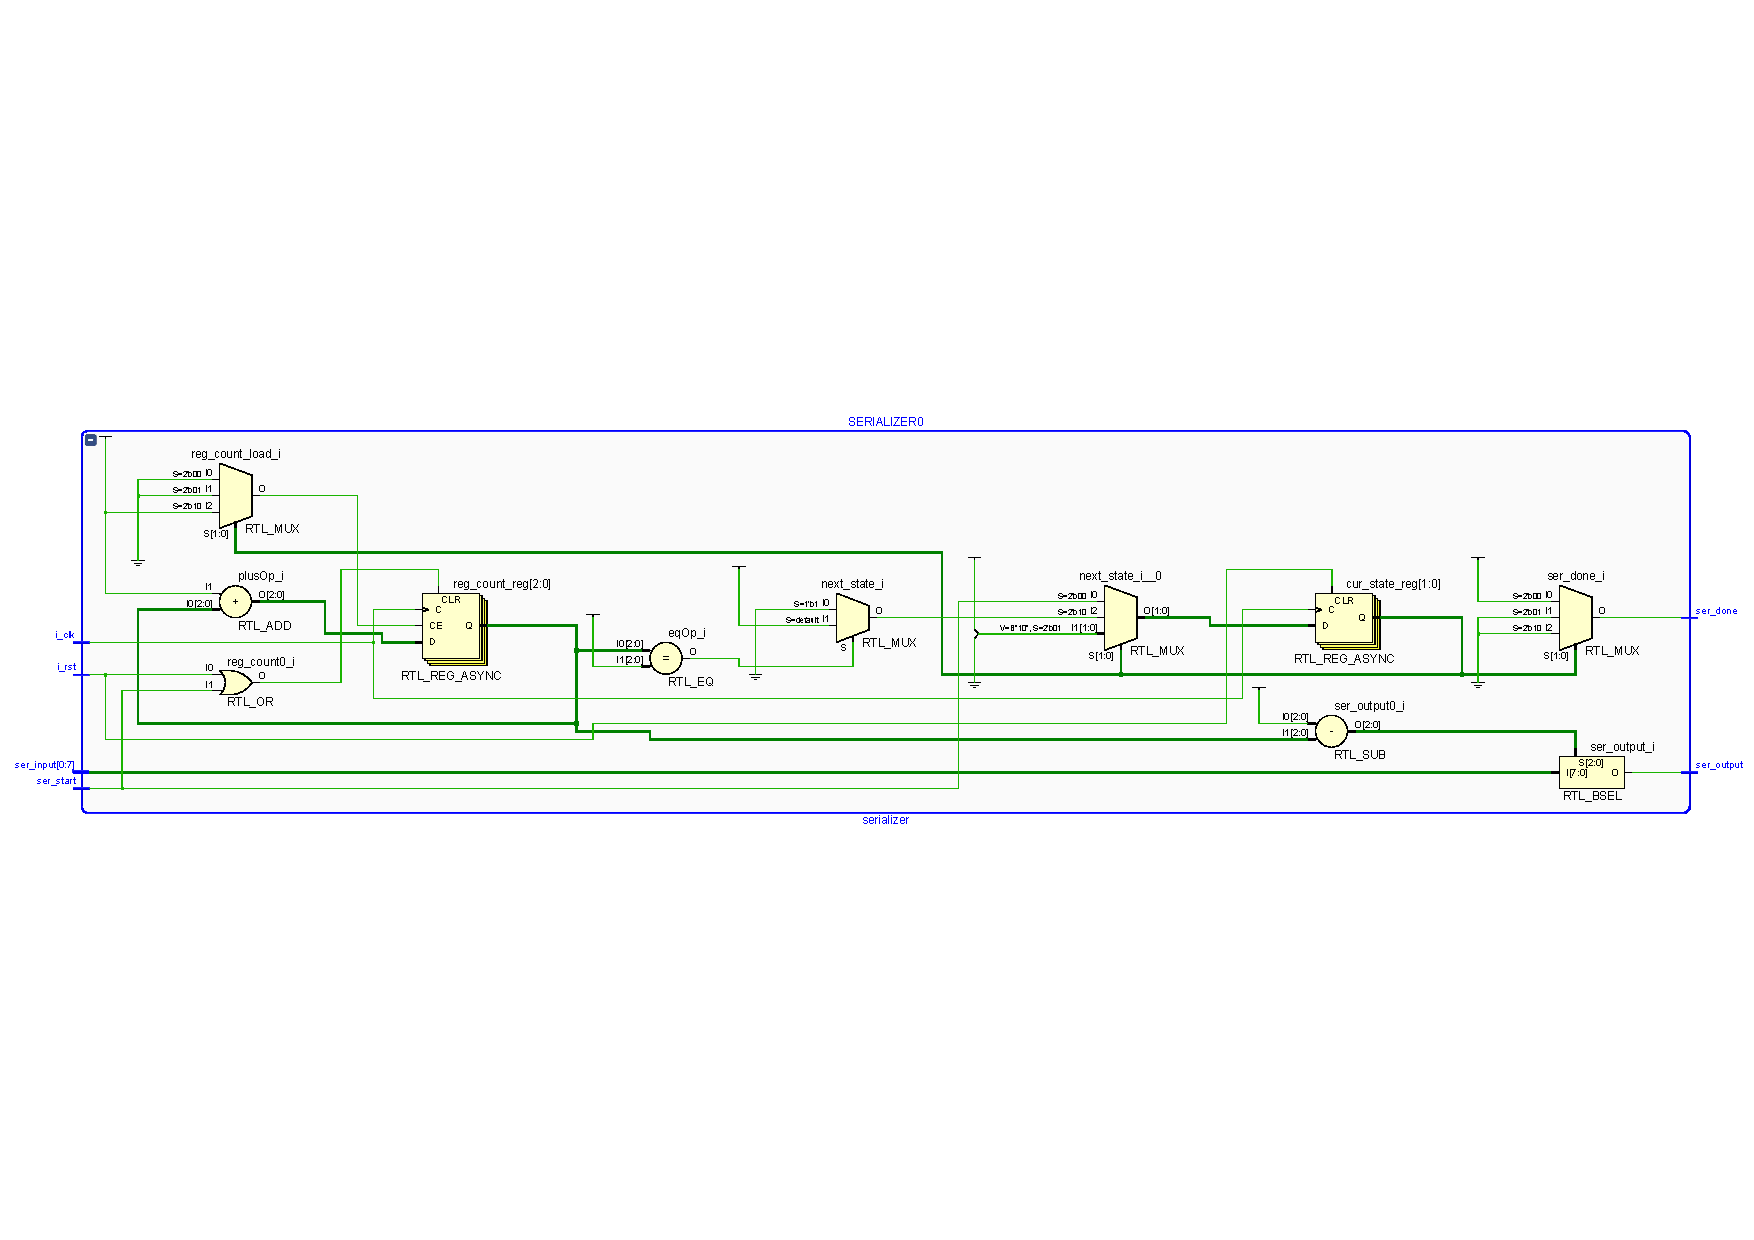
\includegraphics[scale = 0.75]{schematics/serializer.pdf}

Al segnale di \texttt{start} della serializzazione il componente passa dallo stato \textit{STOPPED} allo stato attivo. Quando il componente è attivo produce in uscita per \texttt{due clicli di clock} \textit{n-esimo} bit del segnale in ingresso, incrementando poi il contatore per produrre in uscita l'\textit{n+1 esimo} bit del byte in ingresso nei prossimi due cicli di clock. La serializzazione termina quando il contatore interno raggiunge il valore \texttt{111}: il registro viene incrementato tornando quindi a \texttt{0} ma il serializzatore torna nello stato \texttt{STOPPED}, che alza il segnale di \texttt{done} a \texttt{1}.

Il flusso in uscita ha periodo di due cicli di clock in quanto al convolutore server produrre due bit sequenzialmente in uscita per ogni bit in entrata. In questo modo la velocità di serializzazione è ridotta della metà ma il convolutore riesce a produrro il flusso risultante sullo stesso ciclo di clock della macchina.

%----------------------------------------------------------------------------------------
%	RISULTATI SPERIMENTALI
%----------------------------------------------------------------------------------------

\chapter{Risultati sperimentali}



%----------------------------------------------------------------------------------------
%	CONCLUSIONE
%----------------------------------------------------------------------------------------

\chapter{Conclusione}


\end{document}